%%%--------------------------------------------------------------------------------------------
\documentclass[a4paper, doc, natbib]{apa6}
\usepackage[english]{babel}
\usepackage[utf8x]{inputenc}
\usepackage{mathtools}
\usepackage{amssymb}
\usepackage{graphicx}
\usepackage[colorinlistoftodos]{todonotes} 
\usepackage{etoolbox}

% \usepackage{lineno}

\title{The Effect of Episodic Retrieval on Inhibition in Task Switching}
\shorttitle{Episodic Retrieval \& Inhibition}
\author{James A. Grange, Agnieszka W. Kowalczyk, and Rory O'Loughlin}
\affiliation{School of Psychology, Keele University, UK}

\note{{\bf Word Count:} 7,125 (Main body \& references, not including abstract.)}
% 577 words in references.
% \note{{\bf Under Review---Please, no direct quotes.}}

% command to insert editing comments or track changes
\newcommand{\jg}[1]{\textcolor{blue}{$^{\textrm{}}${#1}}}

%command for R symbol
\newcommand{\R}{R}

\authornote{Please address correspondence to James A. Grange, School of Psychology, Dorothy Hodgkin Building, Keele University, Keele, UK, ST5 5BG. Email: grange.jim@gmail.com. All raw data and analysis code are available to download at http://bit.ly/1P5cd0G.}

\leftheader{Grange, Kowalczyk, \& O'Loughlin}


\abstract{Inhibition in task switching is inferred from n--2 repetition costs: the observation that AB$A$ task switching sequences are responded to slower than CB$A$ sequences. This is thought to reflect the persisting inhibition of task A, which slows re-activation attempts. \cite{Mayr2002} reported an experiment testing a critical non-inhibitory account of this effect, namely episodic retrieval: If the trial parameters for task A match across an ABA sequence, responses should be facilitated due to priming from episodic retrieval; a cost would occur if trial parameters mismatch. In a rule-switching paradigm, Mayr reported no significant difference in n--2 repetition cost when the trial parameters repeated or switched across an ABA sequence, in clear contrast to the episodic retrieval account. What remains unclear is whether successful episodic retrieval \emph{modulates} the n--2 repetition cost. Across three experiments---including a close replication of Mayr (2002)---we find clear evidence of reduced n--2 task repetition costs when episodic retrieval is controlled. We find that the effect of episodic retrieval on the n--2 task repetition cost is increased when the cue--task relationship is made more abstract, suggesting the effect is due to interference in establishing the relevant attentional set. We also demonstrate that the episodic retrieval effect is not influenced by retrieval of low-level, perceptual, elements. Together, the data suggest the n--2 task repetition cost---typically attributable to an inhibitory mechanism---is largely explained by episodic retrieval effects.} 


\keywords{Task switching; inhibition, n--2 repetition cost, episodic retrieval, cognitive control}

\begin{document}
\maketitle

%----------------------
Stimuli in the human environment typically afford more than one action. Sat at a computer, for example, there are many tasks that could be performed, such as writing a manuscript, checking the weather, or playing a game of online chess. In order to act in a goal-directed manner, humans must be able to \emph{select} the relevant task (writing a paper) in the face of competing tasks (playing chess), and maintain this task in an active state so that it can be performed. However, such \emph{stable} task representations must also be \emph{flexible}, so that they can be removed when the goals change (such as when the phone rings). This tension between the need for stability and flexibility of task representations has been called the \emph{stability--flexibility dilemma} \citep{Goschke2000}. 

How the cognitive system solves the stability--flexibility dilemma has been studied using the task switching paradigm \citep{Grange2014a,Kiesel2010,Vandierendonck2010}, wherein participants have to make speeded responses to simple cognitive tasks. For example, participants might be presented with number stimuli, and be asked to switch between judging whether the stimulus is odd/even or lower/higher than five. One cognitive process thought to be essential for task switching performance is the inhibition of competing tasks. Evidence for inhibition comes from the backward inhibition paradigm \citep{Koch2010, Mayr2000}, where participants are required to switch between three tasks (A, B, and C).  It is a consistent finding that AB$A$ task switching sequences are performed slower and with less accuracy than CB$A$ sequences. This effect---know as the \emph{n--2 task repetition cost}---is thought to reflect the persisting inhibition of task A in an ABA sequence, which hinders its re-activation in the last trial of the triplet.

The n--2 task repetition cost is important as it is believed to be a good measure of cognitive inhibition as the n--2 task repetition cost appears to be robust against non-inhibitory explanations \citep{Mayr2007}. One potential explanation of the n--2 task repetition cost that does not assume inhibition was explored by \cite{Mayr2002}. This \emph{episodic retrieval} account \citep{Neill1997} suggests (adapted to a task switching context) that when a task has been performed an episodic trace of trial parameters (such as the cue, stimulus characteristics, and the response made) is stored in memory. When this task is cued again, retrieval of the most recent episodic trace occurs. If the parameters of the presented trial differ from that of the retrieved episode (e.g., a different response is required), a mismatch cost occurs relative to if the retrieved episode matches parameters of the current trial (which will prime performance). Thus, according to this account, n--2 task repetition costs reflect a mismatch cost, as trial parameters typically differ between both instances of task A in an ABA sequence.

\cite{Mayr2002} assessed this alternative explanation by developing a paradigm where the match between trial parameters (i.e., the cue, the stimulus, and the response) across an ABA sequence could be manipulated (see Figure \ref{fig:mayrExperiment}). Participants were required to apply a spatial transformation of a target's location according to one of three stimulus--response rules (vertical, horizontal, or diagonal transformations). For example, if the target is in the bottom-left of the display and the current rule is ``vertical'', the correct response would be an upper-left response (as this reflects a vertical transformation of a bottom-left target). The parameters that might be stored in an episodic trace include (at least) the cue presented, the target's location, and the response made. This paradigm is able to test the episodic retrieval account of n--2 task repetition costs because trial parameters can either match or mismatch across n--2 task repetitions\footnote{Note that with one cue per task, the cue for task A will always be the same across an ABA sequence.}. For example, if the target is in the same location for task A across an ABA sequence, the same response will be required (i.e., an n--2 response repetition). In this case, the episodic retrieval account would predict facilitated performance (i.e., an n--2 task repetition \emph{benefit}). An n--2 response switch, however, would produce an n--2 task repetition cost as there is a mismatch between trial parameters and the retrieved episodic trace (i.e., the response required).

\begin{figure}
\begin{center}
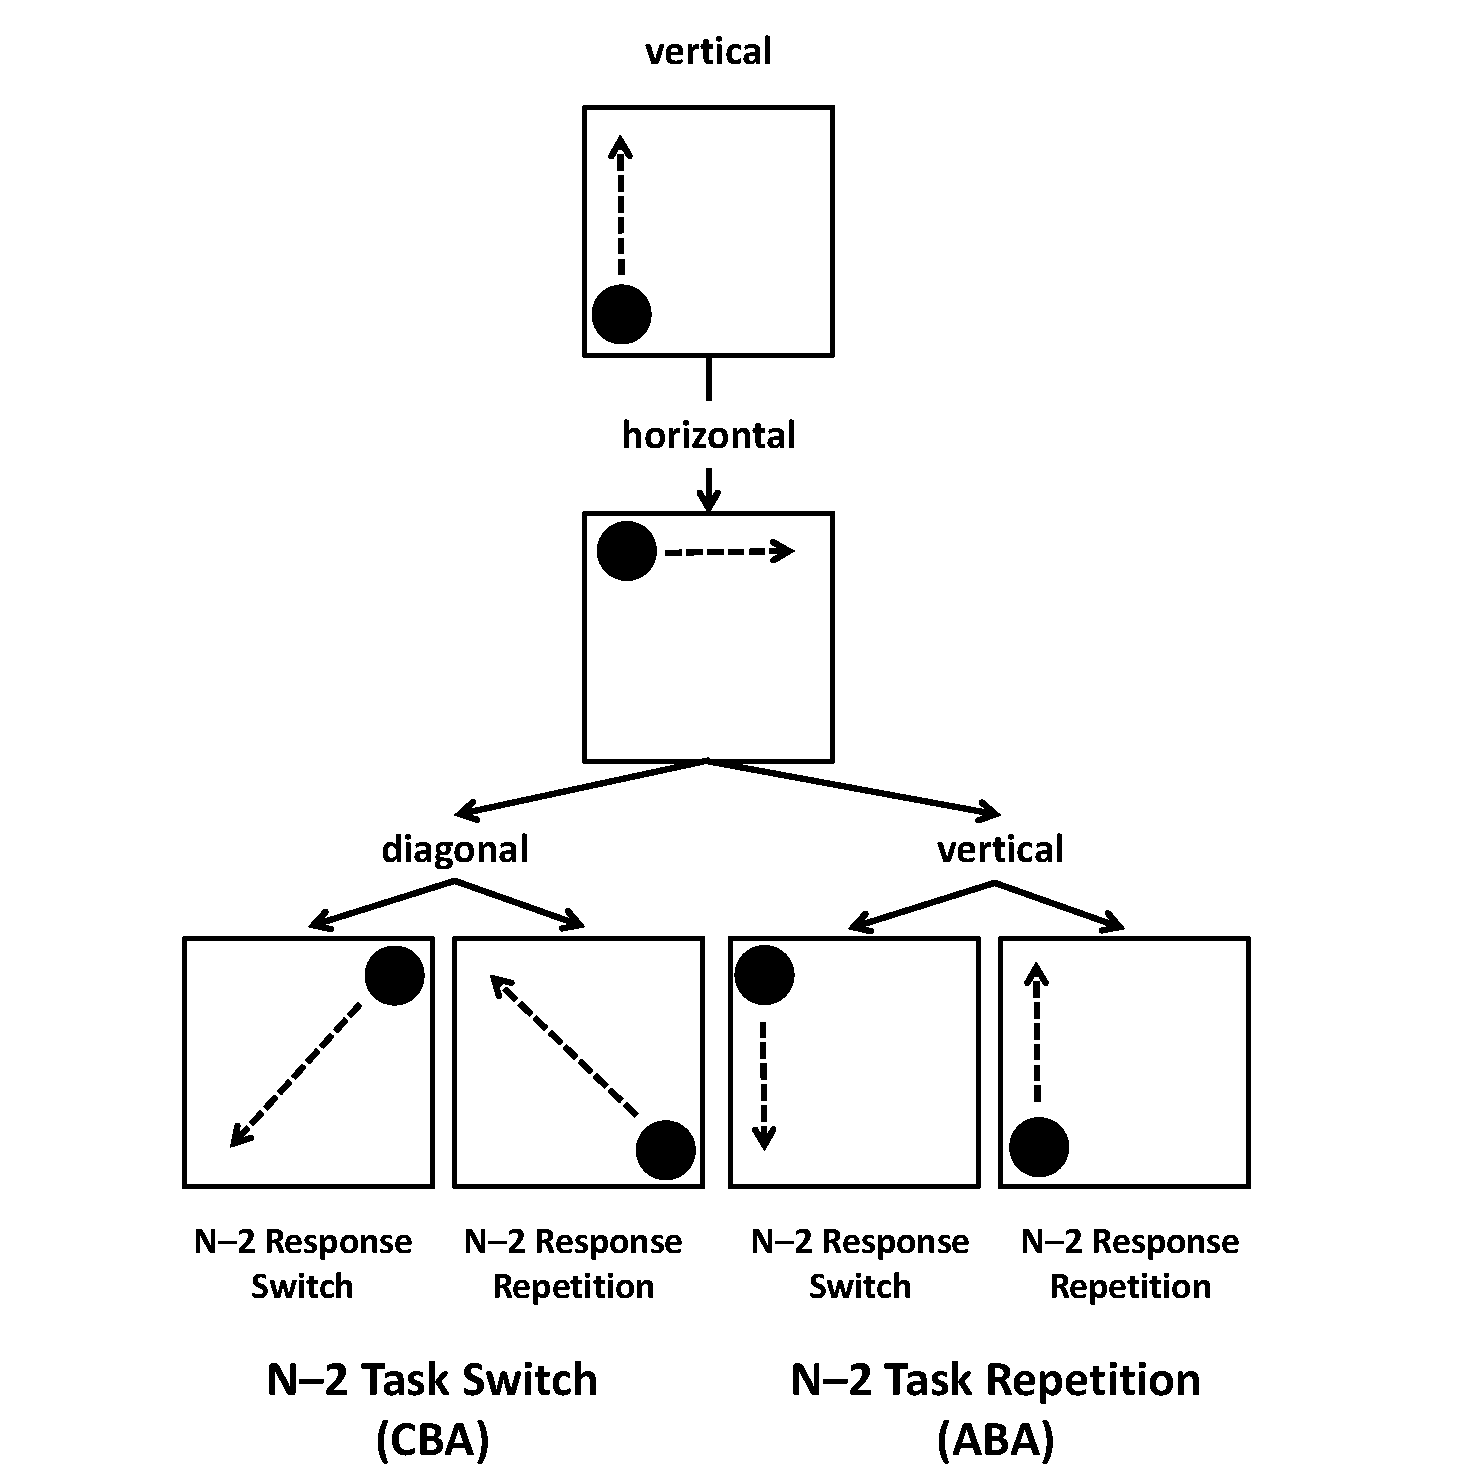
\includegraphics[width = \textwidth]{Images/mayrExperiment.pdf}
\caption{Schematic overview of Mayr's (2002) experimental procedure. The arrows are not displayed to participants, but reflect the spatial transformation required according to the given rule. }
\label{fig:mayrExperiment}
\end{center}
\end{figure}


\cite{Mayr2002} found no statistically significant interaction between n--2 task repetition and n--2 response repetition [$F$(1, 38) = 1.3, $p$ = .26]; that is, there was no significant difference between n--2 task repetition costs for n--2 response repetitions and n--2 response switches. This provides clear evidence against the episodic retrieval account of n--2 task repetition costs, and instead supports the inhibitory account.

\section{The Current Study}
Although Mayr's (2002) study provides clear evidence against episodic retrieval being the \emph{sole} explanation of n--2 task repetition costs, it is not clear from this study whether episodic retrieval has any modulatory effect on this measure of inhibition. Indeed, as Mayr notes in his conclusion, despite the non-significance of the critical interaction, a numerical trend of smaller n--2 task repetition costs for n--2 response repetitions was present in the data. However, the lack of a significant interaction cannot be taken as evidence supporting no modulatory effect, as accepting a null hypothesis cannot be achieved via standard null hypothesis significance testing \citep{Gallistel2009, Wagenmakers2007}; however, evidence in favour of a null hypothesis (given some data) can be obtained using Bayes factors \citep[e.g.,][]{Rouder2009}. The Bayes factor (denoted $BF_{10}$) quantifies the relative evidence provided by the data in favour of an alternative hypothesis (i.e., n--2 task repetition costs are different for response repetitions and response switches) over a null hypothesis (i.e., n--2 task repetition costs are equivalent). 

The Bayes factor for the critical statistical test from Mayr's (2002) study ($BF_{10}$ = 0.315)\footnote{For all Bayes factors reported in this paper we use a non-informative prior on the alternative hypothesis, which is assumed to be distributed as a Cauchy with scaling factor $r$ = 0.707.} suggests that the null hypothesis is about three times more likely than the alternative, given the data, which provides anecdotal-to-moderate support for the null \citep[e.g.,][]{Schoenbrodtinpress}. As this Bayesian analysis does not provide compelling evidence for the null, and given the importance of assessing to what extent (if any) episodic retrieval can influence n--2 task repetition costs in task switching, we were interested in investigating this question further.

The purpose of the current study was to re-examine the evidence for the effect of episodic retrieval on n--2 task repetition costs in a series of Experiments. In Experiment 1, we report a close replication of Mayr's (2002) design, and find that the n--2 task repetition cost is modulated by episodic retrieval. We follow this main finding up in two experiments. In Experiment 2, we manipulate the cue--task transparency---that is, ``\emph{...the degree to which the cue exogenously provides or directly stimulates the relevant [working memory] representations}'' \citep[][p.1004]{Grange2009}. Non-transparent cues require more processing in working memory to establish the relevant attentional set in comparison to transparent cues which require little or no processing in working memory to establish the relevant attentional set \citep[e.g.,][]{Grange2009, Grange2010, Grange2015a, Houghton2009, Mayr2000a}. If the episodic retrieval effect observed in Experiment 1 is caused by interference in working memory establishing a relevant attentional set, then we should observe larger episodic retrieval effects on the n--2 repetition cost under conditions of non-transparent cues; we find strong evidence for such an effect. In a final Experiment, we investigate whether the episodic retrieval effect is sensitive to low-level perceptual details---in particular, task-irrelevant aspects of the stimulus display---and find that it is not. Together, these results provide evidence that the n--2 repetition cost in task switching---typically described as a ``pure'' measure of cognitive inhibition---is heavily influenced by episodic retrieval effects.   

%----------------------
\section{Experiment 1}

In Experiment 1, we wished to replicate critical aspects of Mayr's (2002) design relevant to n--2 task repetitions. As Mayr's study was also interested in exploring to what extent the rule-switching paradigm generated typical task switching effects (such as switch costs, effects of preparation, and effects of the delay between tasks), we made some changes to the original design so that it was more tailored toward assessing n--2 task repetition costs. Specifically, immediate task repetitions were not allowed; it has been shown that including immediate task repetitions reduces the n--2 task repetition cost \citep{Philipp2006}, so we removed this possibility. We also did not manipulate preparation via the cue--stimulus interval, as Mayr reported no effect of this variable on n--2 task repetition costs. Mayr did find that n--2 repetition costs were larger with shorter response--cue intervals (RCI; the time between the response to one trial and the onset of the cue for the next trial), a typical finding for n--2 task repetition costs \citep{Gade2005, Grange2009, Mayr2000}. Therefore, in order to obtain larger n--2 task repetition costs we only used a short RCI. 

\subsection{Method}

\subsubsection{Participants}
All participants were undergraduates at the School of Psychology at Keele University. Participants took part in exchange for partial course credit or a small cash payment (£6). Our final sample comprised 76 participants. The stopping rule utilised a Bayesian sequential analysis, which is detailed in Appendix A. Three additional participants were removed before analysis due to failure to maintain accuracy levels above 90\%.

\subsubsection{Apparatus \& Stimuli}
Stimuli were presented on a 17in. monitor connected to a PC running E-Prime v. 2.0 software. The stimulus display consisted of an 8cm by 8cm square frame. A black circle (diameter = 1 cm.) served as the trial stimulus. Possible cues were the words ``horizontal'', ``vertical'', or ``diagonal'', and were presented in size 22 black Verdanna font directly above the stimulus frame. Responses were collected via a 1-ms. precise USB keyboard.

\subsubsection{Procedure}
On each trial a cue was presented above the frame for 150ms. After this time, the circle stimulus appeared in one of the four corners of the frame. The cue remained on the screen during stimulus presentation. The task required participants to mentally make a spatial transformation of the stimulus' location according to the rule dictated by the task cue, and to make a spatially-congruent response to this translated location. For example, if the stimulus was in the top-right corner of the frame, the participant would need to make a top-left response if the task was ``horizontal'', a bottom-right response if the task was ``vertical'', and a bottom-left response if the task was ``diagonal''. Responses were made on the numerical part of the keyboard, using the ``4'', ``5'', ``1'', and ``2'' keys for top-left, top-right, bottom-left, and bottom-right responses respectively. Participants were asked to respond as quickly and as accurately as possible, using the index finger of their right hand. In between trials, participants were asked to place their finger in the centre of the four response keys. Once a response was registered, the frame was cleared for a response--cue interval of 150ms, after which time a new cue appeared for the next trial. The cue for the next trial was chosen randomly with the constraint that task repetitions could not occur (cf., Mayr, 2002); the stimulus location was chosen randomly with no constraints on each trial. If participants made an error, the word ``Error!'' appeared in red (same size \& font as cues) for 1000ms above the stimulus frame (in the cue's position).

Participants were presented with 16 trials as practice. The practice block was repeated once if the participant made more than four errors. The main experiment presented four blocks of 120 trials. 

\subsubsection{Design}
The experiment manipulated two factors in a fully-related design: \emph{Task Sequence} (n--2 task repetition [ABA] vs. n--2 task switch [CBA]) and \emph{Response Repetition} (n--2 response repetition vs. n--2 response switch). The dependent variables were response time (RT) in milliseconds (ms.) and percent accuracy (\%).


\subsection{Results}
For response time analysis, the first two trials from each block were removed, as were error trials and the two trials following an error. These trials cannot be classified as ABA or CBA sequences. Response times were trimmed by removing all RTs faster than 150ms, as well as any RTs slower than 2.5 standard deviations above the mean for each participant for each cell of the experimental design. Mean RTs and error rates can be seen in Table \ref{tab:Experiment1}.

We present our results using standard null hypothesis significance testing (NHST), as well as Bayesian analysis (Bayes factors). All analysis was conducted using \texttt{R} statistics \citep{RCore2015}. Bayesian analysis utilised the \texttt{BayesFactor} package \citep{Morey2015} and the \texttt{BEST} package \citep{Kruschke2013}.

\begin{table*}[htbp]
\centering
\caption{Response times (RT) in milliseconds (ms) and accuracy (in percent) for ABA and CBA task sequences for response repetitions and response switches in Experiment 1.}
\begin{tabular}{lccccc}
\hline
                    & \multicolumn{5}{c}{Task Sequence}                       \\ \cline{2-6} 
                    & \multicolumn{2}{c}{ABA}   &  & \multicolumn{2}{c}{CBA}  \\ \cline{2-3} \cline{5-6} 
                    & RT (ms)   & Accuracy (\%) &  & RT (ms)  & Accuracy (\%) \\ \hline
N--2 Response Repetition & 1000 (28) & 96.20 (0.39)  &  & 952 (28) & 96.36 (0.39) \\
N--2 Response Switch     & 1050 (29) & 95.02 (0.35)  &  & 964 (28) & 95.81 (0.34) \\ \hline
\end{tabular}
\label{tab:Experiment1}
\end{table*}

\subsubsection{Response Times} 
Response times were analysed via a two factor repeated measures analysis of variance (ANOVA) with the factors \emph{Task Sequence} and \emph{Response Repetition}. There was a significant main effect of Task Sequence, with slower RTs to ABA sequences (1,025ms) than to CBA sequences (958ms), $F$(1, 75) = 94.14, $p$<.001, $\eta_G^2$ = .018. The Bayes factor for this main effect was $BF_{10}$ = 1e+12, which provides substantial support for the presence of n--2 task repetition costs. There was also a significant main effect of Response Repetition, with faster RTs to n--2 response repetitions (976ms) than to n--2 response switches (1,007ms), $F$(1, 75) = 18.21, $p$<.001, $\eta_G^2$ = .004. The Bayes factor for this main effect was $BF_{10}$ = 338.77, which again provides substantial support for the alternative hypothesis. Critically, there was a significant interaction of both factors, $F$(1, 75) = 9.60, $p$<.01, $\eta_G^2$ = .001. The n--2 task repetition cost was 48ms for n--2 response repetitions [$t$(75) = 4.2, $p$<.001; $BF_{10}$ = 271.24] and 86ms for n--2 response switches [$t$(75) = 13.0, $p$<.001; $BF_{10}$ = 7.11e+17]. 

\paragraph{Bayesian Analysis}

The final Bayes Factor for the difference of n--2 task repetition costs for n--2 response repetitions and response switches was $BF_{10}$ = 9.97, which suggests that the alternative hypothesis is about 10 times more likely given the data, which provides strong support that n--2 task repetition costs are influenced by n--2 response repetitions. Due to the theoretical importance of this finding, we provide more detailed Bayesian analysis and robustness checks in Appendix B.

\subsubsection{Accuracy}
Accuracy analysis showed no significant effect of Task Sequence [$F$(1, 75) = 3.36, $p$=.07, $\eta_G^2$ = .006]; the Bayes factor for this main effect was $BF_{10}$ = 0.618, which provides only anecdotal support for the null. The main effect of Response Repetition was significant [$F$(1, 75) = 12.17, $p$<.001, $\eta_G^2$ = .019], suggestive of better accuracy for n--2 response repetitions (96.28\%) than for response switches (95.41\%). The Bayes factor was $BF_{10}$ = 29.66, which provides strong support for the alternative. The interaction was not significant [$F$(1, 75) = 1.32, $p$=.25, $\eta_G^2$ = .003]; the Bayes factor was $BF_{10}$ = 0.238, which provides moderate support for the null hypothesis.

%----------------------
\subsection{Discussion}
Experiment 1 sought to re-examine the evidence for a modulatory effect of episodic retrieval on n--2 task repetition costs in task switching by replicating key aspects of Mayr's (2002) study. In contrast to that study, we found clear evidence of episodic retrieval influencing n--2 task repetition costs in task switching; specifically, n--2 task repetition costs were smaller when the response repeated over an ABA sequence compared to when the response switched. This is in line with episodic retrieval facilitating responding when trial parameters match over an ABA sequence (i.e., for n--2 response repetitions). This finding questions the common interpretation of the n--2 task repetition cost as a ``pure'' measure of task inhibition \citep{Koch2010, Mayr2007}.

%----------------------
\section{Experiment 2}
We wished to follow the findings from Experiment 1 by testing some of the boundary conditions of the effect. In particular, we were interested in whether manipulating the cue--task transparency modulated the observed episodic retrieval effect on the n--2 repetition cost. Recall that non-transparent cues require more processing in working memory to establish the relevant attentional set in comparison to transparent cues which require little or no processing in working memory to establish the relevant attentional set \citep[e.g.,][]{Grange2009, Grange2010, Grange2015a, Houghton2009, Mayr2000a}. In the case of Experiment 1, the word cues are relatively transparent in that the words clearly cue the relevant rule. An example of a non-transparent cue would be arbitrary shapes paired with each task (e.g., a square cue for the ``diagonal'' task). 

Investigating the effect of cue--task transparency was of interest as there is good evidence that non-transparent cues increase the magnitude of the n--2 task repetition cost relative to transparent cues \citep[e.g.,][]{Gade2014, Grange2009, Grange2010, Houghton2009}. Such increases in the n--2 task repetition cost have been interpreted as reflecting an increased need for inhibition. For example \cite{Houghton2009} suggested that non-transparent cues require a process of ``translation'' between the cue and the elements of the task-set required; based on \cite{Mayr2000a}, they suggested this translation involves retrieval of task-set elements from long-term memory and their application in working memory. During a task switch, newly-retrieved elements will conflict with the still-active elements in working memory from the previous task; this interference is resolved by inhibition. Houghton et al. hypothesised that transparent cues do not lead to such interference as the cue provides the desired contents of working memory directly, and as such interference from elements active on the previous trial is minimal. In several studies, Houghton and colleagues \citep{Grange2009, Grange2010, Houghton2009} found evidence that the n--2 task repetition cost is larger for non-transparent cues, and often absent for highly-transparent cues \citep[but see][for a discussion on interpreting null n--2 task repetition costs]{Grange2013}.  

However, given the findings of our Experiment 1, this pattern of data could also be explained under a model of episodic retrieval being influenced by cue transparency, rather than inhibition per se. For example, if the larger n--2 task repetition cost under conditions of episodic mismatch from Experiment 1 was occurring due to conflict between the task-set elements retrieved from episodic memory (from n--2) and the current task parameters in working memory, then reducing the need for working memory in establishing the currently-relevant task-set should reduce this interference. That is, with highly-transparent cues, the need for working memory processing to establish the relevant attentional set is reduced as the cue provides the necessary elements to perform the task successfully; therefore, the parameters retrieved from episodic memory will not interfere with anything. 

Under this hypothesis, the effect of episodic retrieval on the n--2 task repetition cost should be greater under conditions of non-transparent cues. If such a pattern is found, it questions the conclusion that reduced cue-transparency increases the need for inhibition; instead, it would suggest that cue-transparency is influencing episodic interference in working memory. 

To test this, we performed a conceptual replication of Experiment 1, but changed the nature of the task cue in two (within-subject) conditions (see Figure \ref{fig:cues_Experiment2}): In the ``shape'' cue condition, the cues were non-transparent, having no pre-experimental association with the task rules, for example a square cue indicating the ``diagonal'' judgment. In contrast, the ``arrow'' cues condition, the cue provides a direct sample of the response rules relevant for the current trial. For example, the ``vertical'' judgment is cued by two up--down arrows. We predicted that the effect of episodic retrieval on the n--2 task repetition cost would be greater for the Shape cues compared to the Arrow cues. 

\subsection{Method}
\subsubsection{Participants}
The stopping rule for Experiment 2 is detailed in Appendix A. All participants were from the same pool as Experiment 1, receiving the same compensation. None had taken part in Experiment 1. Our final sample consisted of 66 participants.

\subsubsection{Apparatus \& Stimuli}
The apparatus was identical to Experiment 1. The stimulus frame and stimulus object was identical to Experiment 1, but we did not use the word cues. Instead, participants were presented with ``arrow'' cues in one half of the experiment, and ``shape'' cues in the other half. The cues were presented in the centre of the stimulus frame. The cues are shown in Figure \ref{fig:cues_Experiment2}. For the shape cues, a hexagon cued the vertical judgement, a triangle cued the horizontal judgement, and a square cued the diagonal judgement. The arrow cues visually dictated the response rule: vertical arrows cued the vertical judgement, horizontal arrows cued the horizontal judgement, and diagonal arrows cued the diagonal judgement. All cues were 2.5cm in width and height.


\begin{figure*}
\begin{center}

\includegraphics[width = \textwidth]{Images/experiment_2_cues.png}
\caption{Cues from Experiment 2 for each of the three judgements (vertical, horizontal, and diagonal).}
\label{fig:cues_Experiment2}
\end{center}
\end{figure*}


\subsubsection{Procedure}
The Experiment was in two halves, with different cue-types presented in each half. Order of cue presentation in each half was counterbalanced across participants. For each half, participants learned the cue--task pairings, and were presented with a practice session consisting of 16 trials, which was repeated once if the participant made than four errors. The experimental section of each half consisted of three blocks of 120 trials. The trial procedure and response requirements were the same as Experiment 1. 

\subsubsection{Design}
The experiment manipulated three factors in a fully-related design: \emph{Cue-Type} (arrow cues vs. shape cues), \emph{Task Sequence} (n--2 task repetition [ABA] vs. n--2 task switch [CBA]) and \emph{Response Repetition} (n--2 response repetition vs. n--2 response switch). The dependent variables were response time (RT) in milliseconds (ms.) and percent accuracy (\%).

\subsection{Results}
The data trimming was identical to Experiment 1. Mean RTs and errors are presented in Table \ref{tab:Experiment2}.

\subsubsection{Response Times}
Response times\footnote{All of the response time analysis was re-analysed using log(RT) as the dependent variable, which produced qualitatively similar results. This transformation was analysed as there was a large discrepancy in mean response time for arrow cues and shape cues, and as such, interaction effects could have been artificially amplified.} were analysed via a three factor repeated measures ANOVA with the factors \emph{Cue-Type, Task Sequence} and \emph{Response Repetition}. There was a significant main effect of Cue-Type, with faster RTs to arrow cues (720ms) than to shape cues (1067ms), $F$(1, 65) = 247.98, $p$<.001, $\eta_G^2$ = .42. There was also a main effect of Task Sequence, with slower RTs to ABA sequences (916ms) than to CBA sequences (871ms), $F$(1, 65) = 61.75, $p$<.001, $\eta_G^2$ = .012. There was also a main effect of Response Repetition, with faster RTs to response repetitions (878ms) than to response switches (909ms), $F$(1, 65) = 24.53, $p$<.001, $\eta_G^2$ = .006.


\begin{table*}[htbp]
\centering
\caption{Response times (RT) in milliseconds (ms) and accuracy (in percent) for ABA and CBA task sequences for response repetitions and response switches for both cue types in Experiment 2.}
\begin{tabular}{lllllll}
\hline
         &                          & \multicolumn{5}{c}{Task Sequence}                        \\ \cline{3-7}

         &                          & \multicolumn{2}{c}{ABA}   &  & \multicolumn{2}{c}{CBA}   \\\cline{3-4}
\cline{6-7}

Cue Type &                          & RT (ms)   & Accuracy (\%) &  & RT (ms)   & Accuracy (\%) \\ \hline
Arrows   & N--2 Response Repetition & 722 (22)  & 98.05 (0.29)  &  & 709 (20)  & 96.64 (0.40)  \\
         & N--2 Response Switch     & 739 (20)  & 96.36 (0.32)  &  & 709 (20)  & 97.49 (0.22)  \\
         &                          &           &               &  &           &               \\
Shapes   & N--2 Response Repetition & 1053 (29) & 96.90 (0.40)  &  & 1027 (30) & 95.75 (0.49)  \\
         & N--2 Response Switch     & 1148 (29) & 94.20 (0.47)  &  & 1039 (30) & 96.66 (0.30) \\
\hline
\end{tabular}
\label{tab:Experiment2}
\end{table*}


Replicating previous work (Grange \& Houghton, 2009, 2010; Houghton et al., 2009), there was a significant interaction of Cue-Type and Task Sequence [$F$(1, 65) = 15.85, $p$<.001, $\eta_G^2$ = .003], with smaller n--2 task repetition costs for the more ``transparent'' arrow cues (22ms) than for the more ``non-transparent'' shape cues (68ms). Cue-Type also interacted with Response Repetition [$F$(1, 65) = 16.07, $p$<.001, $\eta_G^2$ = .003]: The difference of slower RTs for response switches compared to response repetitions was smaller for arrow cues (8ms) than for the shape cues (53ms).

Replicating Experiment 1, we also found a significant interaction of Task Sequence and Response Repetition [$F$(1, 65) = 14.87, $p$<.001, $\eta_G^2$ = .004.]: n--2 repetition costs were smaller for response repetitions (20ms) than for response switches (70ms). This replication provides converging evidence that the n--2 task repetition cost is reduced under conditions of an episodic match from n--2. 

Pertinent to the current Experiment's aims, we also found a significant interaction between all three factors, $F$(1, 65) = 8.88, $p$<.01, $\eta_G^2$ = .002. This suggests that the difference in n--2 task repetition cost for response repetitions and response switches varied between Cue-Type. This three-way interaction is depicted in the upper panel of Figure \ref{fig:Experiment2}. A simplified depiction of this interaction is depicted in the lower panel of Figure \ref{fig:Experiment2}, where we plot the n--2 task repetition cost as the dependent variable. As is clear, the difference between the n--2 task repetition cost for response repetitions and response switches was larger for the non-transparent shape cues. That is, episodic retrieval appeared to have a larger modulatory effect for the shape cues, as predicted.   

\begin{figure*}
\begin{center}
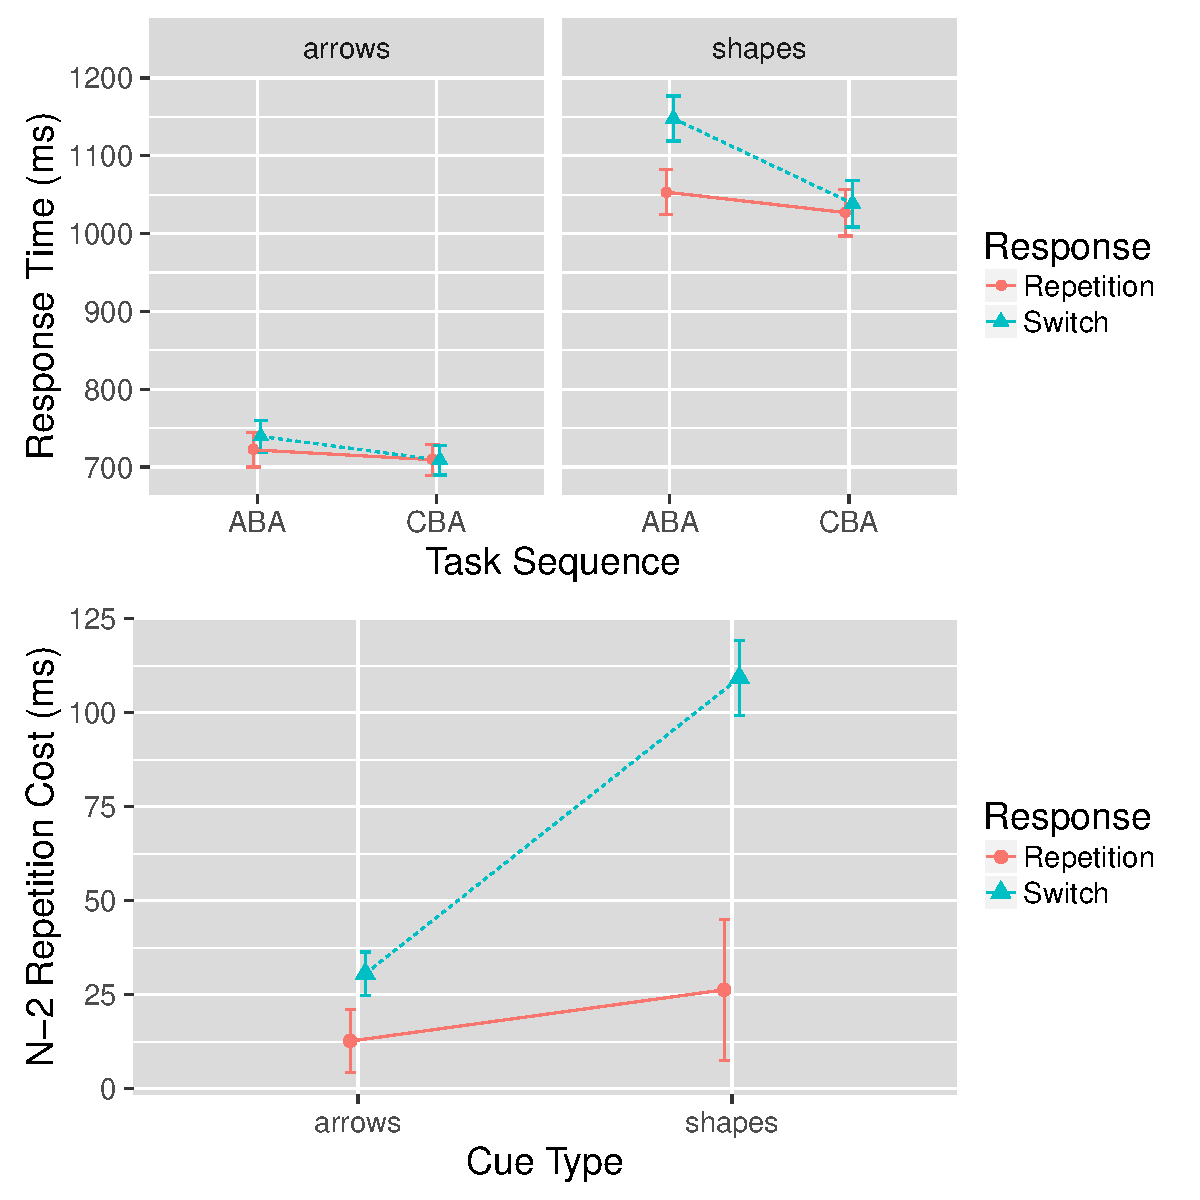
\includegraphics[width = \textwidth]{Images/all_rts_Experiment2.pdf}
\caption{Data from Experiment 2. The upper panel depicts the three-way interaction of Cue-Type (arrows vs. shapes), Task Sequence, and Response Repetition for mean response time (in milliseconds, ms). The lower panel depicts the same data expressed with N--2 task repetition costs as the dependent variable, for both cue types as a function of response repetition and response switch from n--2 to n. Error bars denote +/- 1 standard error around the mean.}
\label{fig:Experiment2}
\end{center}
\end{figure*}

\paragraph{Bayesian Analysis}
See Appendix A for details of the Bayesian model comparison process. We modelled the data in the lower portion of Figure \ref{fig:Experiment2}, with n--2 task repetition cost as the dependent variable. The ``full'' model---i.e., two main effects (Cue-Type and Response Repetition) plus their interaction---had a Bayes factor of 1,236,317. The next-best model was the model with two main effects---Cue-Type and Response Repetition---with a Bayes factor of 156,707. Thus, the $BF_{10}$ for the full interaction model was 1,236,317 / 156,707 = 7.89, suggesting the evidence in support of the interaction of Cue-Type and Response Repetition is about 8 times greater than the next-best model. This provides moderate support for this model. Thus, the NHST and Bayesian analysis both support the conclusion that the episodic retrieval effect on the n--2 task repetition cost is greater for non-transparent cues, as predicted. 


\subsubsection{Accuracy}
For the accuracy data, there was a significant main effect of Cue-Type, with more accurate responses to arrow cues (97.13\%) compared to shape cues (95.88\%), $F$(1, 65) = 16.57, $p$<.001, $\eta_G^2$ = .042. The main effect of Task Sequence was not significant, $F$(1, 65) = 1.38, $p$=.244, $\eta_G^2$ = .002. There was a main effect of Response Repetition, with more correct responses to response repetitions (96.84\%) compared to response switches (96.18\%), $F$(1, 65) = 12.81, $p$<.001, $\eta_G^2$ = .012.

The interaction of Cue-Type and Task Sequence was not significant, $F$(1, 65) = 3.79, $p$=.056, $\eta_G^2$ = .004, nor was the interaction of Cue-Type and Response Repetition, $F$(1, 65) = 1.33, $p$=.254, $\eta_G^2$ = .002. There was a significant interaction between Task Sequence and Response Repetition, $F$(1, 65) = 51.99, $p$<.001, $\eta_G^2$ = .061, indicative of different n--2 task repetition costs for response repetitions and response switches. The n--2 task repetition cost---calculated as $\%Accuracy_{ABA}$ -- $\%Accuracy_{CBA}$---for response switches was --1.79\%, but there was an n--2 task repetition \emph{benefit} of 1.28\% for response repetitions. The three way interaction was not significant, $F$(1, 65) = 1.69, $p$=.199, $\eta_G^2$ = .002.

\subsection{Discussion}
Experiment 2 replicated the finding from Experiment 1 of increased n--2 task repetition costs under conditions of n--2 response switches (i.e., episodic mismatches). In addition, this effect was larger when the cue--task relationship was relatively non-transparent (i.e., the Shape cues). We suggest that the transparent Arrow cues minimise the role of working memory in establishing the relevant attentional set, and as such, elements retrieved from episodic memory interfere less with ongoing processing. This finding localises the episodic retrievel effect on n--2 task repetition costs to interference during establishing the relevant attentional set for current task performance.

The current finding also has implications for previous work suggesting that cue--task transparency influences the degree of inhibition deployed during task switching \citep{Grange2009, Grange2010, Grange2015a, Houghton2009}. Cue--task transparency in Experiment 2 only appeared to influence the n--2 task repetition cost under conditions of n--2 response switches; cue--task transparency had little influence on the n--2 task repetition cost under conditions of n--2 response repetitions. If we assume the latter condition is a better measure of ``pure'' inhibition---in the sense that the n--2 task repetition cost here is not influenced by episodic retrieval---we can see that cue--task transparency is not having a large effect on inhibition. We return to the implications of this finding in the General Discussion. 

%----------------------
\section{Experiment 3}
In the final Experiment, we wished to understand whether the observed episodic retrieval effect in Experiments 1 and 2 was sensitive to low-level perceptual details of the stimulus display. In Experiments 1 and 2, the identity of the stimulus was always task-irrelevant; what was relevant was the location of the stimulus. Therefore, we were interested in whether the facilitatory performance we find for n--2 task repetition costs under conditions of n--2 response repetitions was due to low-level perceptual matching of the stimulus identity between the episodic trace retrieved and the current stimulus display, or a matching between more ``high-level'' representations, such as the stimulus location and the response required. Finding that the episodic retrieval effect is not sensitive to low-level, task-irrelevant, perceptual properties of the task would suggest that what is being retrieved from episodic memory during task switching are exclusively task-relevant elements of task performance. 

To this end, we designed an experiment which varied the novelty of the task-relevant stimulus on each trial. The paradigm was very similar to the ``Shape'' condition of Experiment 2, but the stimulus was always a letter. In the ``Match'' condition, the stimulus was always the letter ``A''; thus, there is always a perceptual match of the stimulus identity between n--2 and n. In the ``Mismatch'' condition, the stimulus was randomly drawn from the set ``A--Z''; thus, in this condition, the probability of a perceptual match of the stimulus identity between n--2 and n is drastically reduced. 

If the episodic retrieval effect observed thus far is sensitive to low-level, task-irrelevant, properties of the stimulus display, we should find a larger episodic facilitatory effect in the Match condition, as this is the only condition where such details match across n--2 to n. If, however, the effect is due to retrieval of task-relevant, ``high-level'' representations---such as stimulus location and the response executed---we should find similar effects of episodic retrieval in both conditions.

\subsection{Method}
\subsubsection{Participants}
The stopping rule for Experiment 3 is detailed in Appendix A. All participants were from the same pool as Experiments 1 and 2, receiving the same compensation. None had taken part in either of these Experiments. Our final sample consisted of 25 participants.

\subsubsection{Apparatus \& Stimuli}
The apparatus was identical to Experiments 1 and 2. The stimulus frame was also identical to Experiment 1, but different stimuli were used. Instead of circles, letters served as stimuli, presented in Verdana font approximately 1cm in height and width. In one condition---the \emph{Match} condition---the stimulus was always the letter ``A''. In the other condition---the \emph{Mismatch} condition---the stimulus was selected from the letters A--Z. The cues were the shape cues used from Experiment 2, and were presented in the centre of the stimulus frame. A hexagon cued the vertical judgment, a triangle cued the horizontal judgment, and a square cued the diagonal judgment. All cues were 2.5cm in width and height.


\subsubsection{Procedure}
The Experiment was in two halves, with different stimulus conditions presented in each half. In the Match condition, the same letter was presented as the stimulus on all trials (the letter ``A'' for all participants). In the Mismatch condition, the stimulus was randomly selected (with replacement) from the set A--Z. Participants were informed that the identity of the stimulus was always irrelevant, and that they were to always respond based on the current task and the location of the stimulus.

The ordering of stimulus condition was counterbalanced across participants. Participants were presented with a practice session in both halves, consisting of 16 trials which was repeated once if the participant made than four errors. The experimental section of each half consisted of three blocks of 120 trials. The trial procedure and response requirements were the same as Experiment 1. 

\subsubsection{Design}
The experiment manipulated three factors in a fully-related design: \emph{Stimulus Condition} (match vs. mismatch), \emph{Task Sequence} (n--2 task repetition [ABA] vs. n--2 task switch [CBA]) and \emph{Response Repetition} (n--2 response repetition vs. n--2 response switch). The dependent variables were response time (RT) in milliseconds (ms.) and percent accuracy (\%).

\subsection{Results}
The data trimming was identical to Experiments 1 and 2, with the exception that trials in the Mismatch condition in which a stimulus repeated from the previous trial or from the trial at n--2 were removed. Mean RTs and errors are presented in Table \ref{tab:Experiment3}.

\begin{table*}[htbp]
\centering
\caption{Response times (RT) in milliseconds (ms) and accuracy (in percent) for ABA and CBA task sequences for response repetitions and response switches for both cue types in Experiment 3.}
\begin{tabular}{lllllll}
\hline
         &                          & \multicolumn{5}{c}{Task Sequence}                        \\ \cline{3-7}

         &                          & \multicolumn{2}{c}{ABA}   &  & \multicolumn{2}{c}{CBA}   \\\cline{3-4}
\cline{6-7}

Stimulus &                          & RT (ms)   & Accuracy (\%) &  & RT (ms)   & Accuracy (\%) \\ \hline
Match   & N--2 Response Repetition & 1074 (51) & 96.99 (0.88)  &  & 1042 (51)  & 97.55 (0.49)  \\
         & N--2 Response Switch     & 1124 (51)  & 96.60 (0.42)  &  & 1038 (49)  & 97.86 (0.56)  \\
         &                          &           &               &  &           &               \\
Mismatch   & N--2 Response Repetition & 1075 (50) & 95.63 (0.69)  &  & 1047 (56) & 97.62 (0.72)  \\
         & N--2 Response Switch     & 1131 (49) & 95.47 (0.69)  &  & 1002 (45) & 97.06 (0.38) \\
\hline
\end{tabular}
\label{tab:Experiment3}
\end{table*}


\subsubsection{Response Times}
Response times were analysed via a three factor repeated measures ANOVA with the factors \emph{Stimulus Condition}, \emph{Task Sequence}, and \emph{Response Repetition}. The main effect of Stimulus Condition was not significant, $F$(1, 24) = 0.01, $p$ = .924, $\eta_G^2$ < .001. There was a main effect of Task Sequence, with slower RTs to ABA sequences (1101ms) than to CBA sequences (1032ms), $F$(1, 24) = 35.74, $p$ < .001, $\eta_G^2$ = .019. The main effect of Response Repetition was not significant, $F$(1, 24) = 1.20, $p$ = .283, $\eta_G^2$ < .001.

Stimulus Condition did not interact with Task Sequence [$F$(1, 24) = 0.87, $p$ = .362, $\eta_G^2$ < .001] or Response Repetition [$F$(1, 24) = 0.66, $p$ = .426, $\eta_G^2$ < .001]. Replicating the first two Experiments, Task Sequence interacted with Response Repetition, $F$(1, 24) = 17.04, $p$ < .001, $\eta_G^2$ = .006: n--2 task repetition costs were smaller for response repetitions (29ms) than for response switches (108ms). This provides converging evidence that the n--2 repetition cost is reduced under conditions of an episodic match from n--2. 

Importantly for the current study, the three-way interaction was not significant, $F$(1, 24) = 1.07, $p$ = .311, $\eta_G^2$ < .001. This three-way interaction is depicted in the upper panel of Figure \ref{fig:Experiment3}. A simplified depiction of this interaction is depicted in the lower panel of Figure \ref{fig:Experiment3}, where we plot the n--2 task repetition cost as the dependent variable. There is no clear variation of the episodic-retrieval effect on n--2 task repetition costs under conditions of stimulus matching or mismatching.  

\paragraph{Bayesian Analysis}
See Appendix A for details of the Bayesian model comparison process. We modelled the data in the lower portion of Figure \ref{fig:Experiment3}, with n--2 task repetition cost as the dependent variable. The ``full'' model---i.e., two main effects (Stimulus Condition and Response Repetition) plus their interaction---had a Bayes factor of 24.17. The best model was the model with Response Repetition as the only main effect, with a Bayes factor of 151.10. Thus, the $BF_{10}$ for the full interaction model was 24.17 / 151.10 = 0.16, suggesting the evidence against the interaction of Stimulus Condition and Response Repetition is about 6.25, which constitutes moderate evidence against this model. Thus, the NHST and Bayesian analysis both support the conclusion that, whilst the n--2 task repetition cost is modulated by episodic retrieval, the effect is similar for both Stimulus Conditions. 

\subsubsection{Accuracy}
For the accuracy data, there was no significant main effect of Stimulus Condition, $F$(1, 24) = 2.46, $p$ = .130, $\eta_G^2$ = .017. There was a significant main effect of Task Sequence, with less accurate response to ABA sequences (96.17\%) than to CBA sequences (97.52\%), $F$(1, 24) = 14.64, $p$ < .001, $\eta_G^2$ = .046. The main effect of Response Repetition was not significant, $F$(1, 24) = 0.58, $p$ = .452, $\eta_G^2$ = .001.

None of the interactions were significant: Stimulus Condition by Task Sequence, $F$(1, 24) = 1.33, $p$ = .260, $\eta_G^2$ = .005; Stimulus Condition by Response Repetition, $F$(1, 24) = 0.23, $p$ = .638, $\eta_G^2$ < .001; Task Sequence by Response Repetition, $F$(1, 24) = 0.05, $p$ = .821, $\eta_G^2$ < .001. The three-way interaction was also not significant, $F$(1, 24) = 0.62, $p$ = .438, $\eta_G^2$ = .002.

\begin{figure*}
\begin{center}
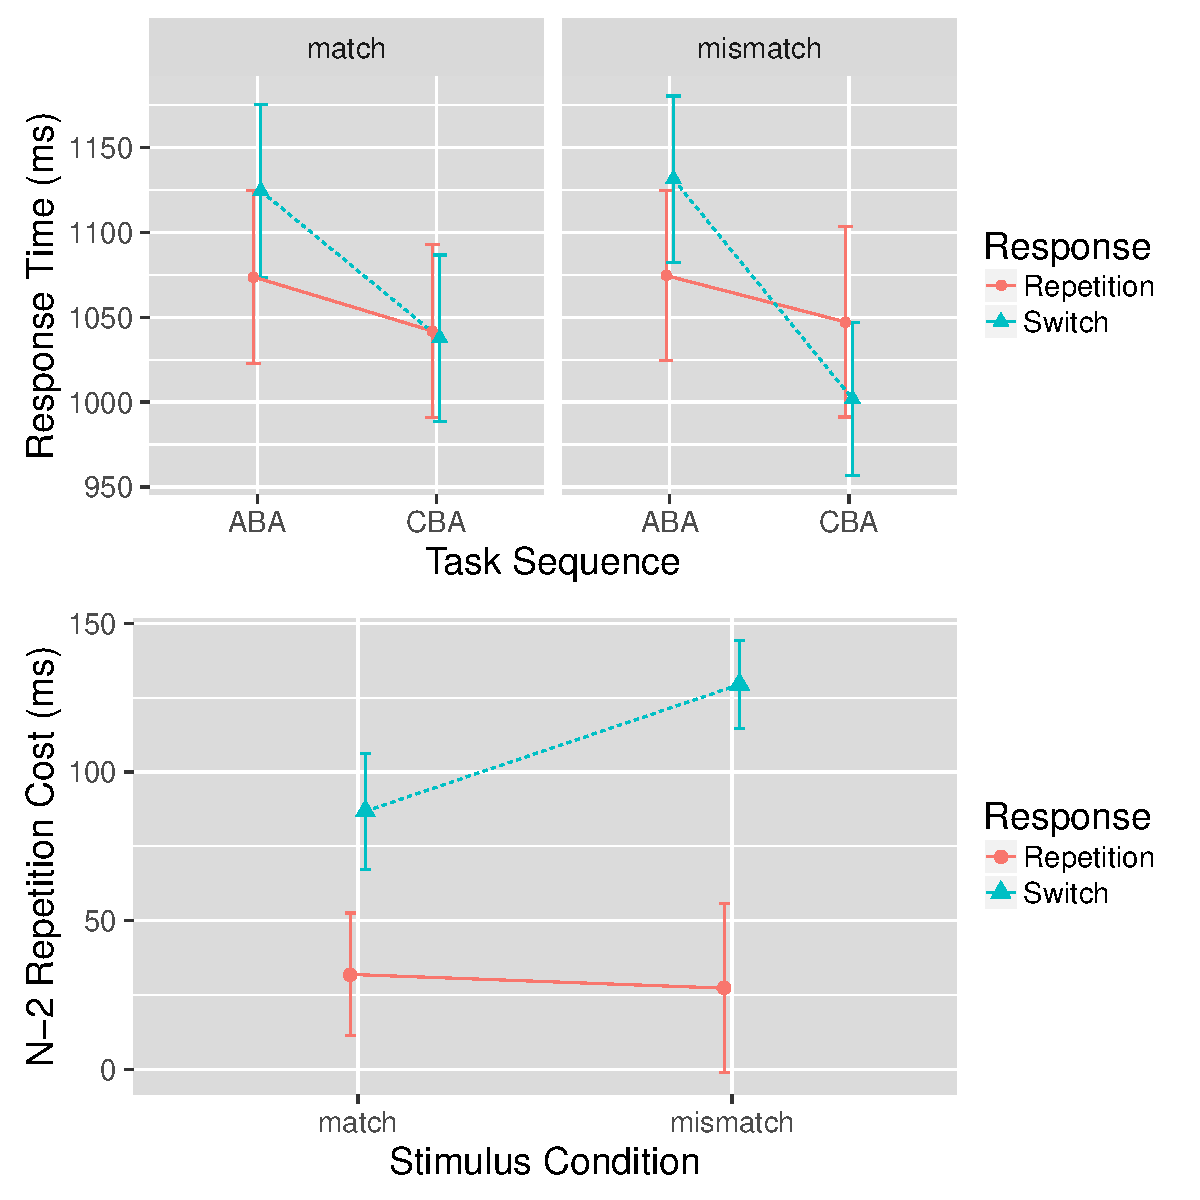
\includegraphics[width = \textwidth]{Images/all_rts_Experiment3.pdf}
\caption{Data from Experiment 3. The upper panel depicts the three-way interaction of Stimulus Condition (match vs. mismatch), Task Sequence, and Response Repetition for mean response time (in milliseconds, ms). The lower panel depicts the same data expressed with N--2 task repetition costs as the dependent variable, for both Stimulus Conditions as a function of response repetition and response switch from n--2 to n. Error bars denote +/- 1 standard error around the mean.}
\label{fig:Experiment3}
\end{center}
\end{figure*}


\subsection{Discussion}
We were interested in whether the effect of episodic retrieval on the n--2 task repetition cost was due to low-level perceptual details of the stimulus display. The results support the conclusion that it is not: The effect of episodic retrieval on the n--2 task repetition cost was similar under conditions of stimulus matching and stimulus mismatching from n--2 to n. These results suggest that the episodic retrieval effect observed in all three experiments can be localised to the retrieval of ``high-level'', task-relevant representations, such as the stimulus location and the response executed. 

%----------------------
\section{General Discussion}
The current study was interested in re-investigating whether---and to what extent---episodic retrieval affects the n--2 task repetition cost, an effect typically ascribed to a ``pure'' measure of task inhibition \citep{Gade2014, Koch2010, Mayr2007}. Across three experiments, we find consistent evidence that the n--2 task repetition cost is increased when there is a mismatch between task-relevant elements from episodic memory of the task from n--2 and the task demands on the current trial. When the trace from n--2 that is retrieved from episodic memory matches the current task demands, the n--2 task repetition cost is significantly reduced. Experiment 2 demonstrated that the effect is larger for less-transparent cue--task relationships, which we suggest provides evidence that localises the episodic retrieval effect to interference during establishing the relevant attentional set in working memory. In Experiment 3 we demonstrated that the effect is not influenced by low-level perceptual properties being retrieved from episodic memory. Rather, the effect appears to be localised to higher-level representations regarding task-relevant stimulus properties and response execution. 

Together, our data suggests that episodic retrieval strongly modulates the n--2 task repetition cost. Therefore, we suggest that the n--2 task repetition cost---as typically measured---is at least a contaminated measure, and should be used with caution. Not controlling for episodic retrieval will bias the estimates of n--2 task repetition costs. 

\subsection{Practical Implications}
This finding has significant practical implications, as the n--2 task repetition cost has garnered much interest with researchers interested in using the n--2 task repetition cost as a measure of inhibitory control. For example, \cite{Whitmer2007} used the n--2 task repetition cost as a measure of inhibition to assess to what extent depressive rumination is associated with deficient inhibitory control, finding a negative correlation between n--2 task repetition costs and rumination tendencies; from this, the authors concluded that rumination is associated with deficits in cognitive inhibition \citep[see also][]{Whitmer2012}. The n--2 task repetition cost has also been used to assess the effects of brain lesions on cognitive inhibition \citep{Mayr2006}, the effect of Parkinson's \citep{Fales2006}, healthy ageing \citep{Lawo2012}, obsessive-compulsive disorder \citep{Moritz2004}, bilingualism \citep{Prior2012}, and others. Our findings would suggest that the results of such studies need reconsideration, as episodic retrieval was not controlled. Therefore, the measures of the n--2 task repetition cost are likely confounded.

Recently, we have reported that the split--half reliability of individual differences in the n--2 task repetition cost is low, by assessing performance on three paradigms typically used in assessing the n--2 task repetition cost \citep{Kowalczykinpress}. This finding is consistent with the notion that the n--2 task repetition cost is not a stable measure of inhibition at the individual difference level, but it is also expected if the n--2 task repetition cost arises due to a mixture of factors (i.e., inhibition plus episodic interference). As episodic retrieval was not controlled in the paradigms used by \cite{Kowalczykinpress}---as is typical in this line of research---one possibility is that the low reliability was caused by the contamination episodic interference brings to the measure. Current work in our lab is assessing whether reliability of the n--2 task repetition cost improves when episodic retrieval is controlled.

\subsection{Theoretical Implications}
There are also theoretical implications of these findings. There is growing evidence that episodic retrieval plays a role in explaining several task switching effects \citep[e.g.,][for a model of task switching based on episodic retrieval]{Altmann2008}. For example, \cite{Altmann2011} provided empirical and theoretical evidence that episodic retrieval can explain the n--1 response-repetition effect in task switching, the observation that task repetition RTs are facilitated when the required response repeats from trial n--1 to the current trial, yet n--1 response repetitions produce a cost for task switches. \cite{Horoufchin2011a} \citep[see also][]{Horoufchin2011} also provided evidence that episodic retrieval can explain the reduction of the task switch cost at longer RCIs \citep[e.g.,][]{Meiran2000a}; the standard explanation for this finding pertains to the decay of task representations in memory slowing task repetition RTs. However, \cite{Horoufchin2011a} provided compelling evidence that this pattern of data can be better explained with reference to an episodic retrieval account: trial-wise variation of the RCI affects the \emph{temporal distinctiveness} of task traces in episodic memory, thus influencing their retrieval probability \citep{Brown2007, Grange2015, Grange2016}. The current work extends this evidence of the role of episodic retrieval influencing task switching effects. As such, theoretical accounts of inhibitory control during task switching will have to take into account the role of episodic retrieval.

As the n--2 task repetition cost has been thought to measure a pure inhibitory mechanism, previous research which has shown a modulation of the n--2 task repetition cost due to some experimental manipulation has been interpreted in terms of the manipulation having an effect on inhibition. For example, \cite{Schuch2003} found that the n--2 task repetition cost is absent if the task at n--1 did not require a response (i.e., a no-go trial). This evidence was used to suggest that inhibition of competing tasks occurs at the response-selection level. Other work has found effects of the cue-type \citep{Arbuthnott2005, Grange2009, Grange2010, Houghton2009}, response--related processes \citep{Philipp2007, Schneider2008}, stimulus-related processes \citep{Sdoia2008}, RCI effects \citep{Gade2005}, and practice effects \citep{Grange2015a, Scheil2016}, among others \citep{Koch2010}. As such, it would be prudent to re-visit these findings and assess to what extent the experimental manipulations were influencing episodic retrieval rather than inhibition. 

For example, the current work has implications for our previous line of research focussing on the effects of cue--transparency on the n--2 task repetition cost \citep{Grange2009, Grange2010, Grange2015a, Houghton2009}. Our previous work has shown consistently that reducing the transparency of the cue--task relationship increases the n--2 task repetition cost. However, Experiment 2 of the current study provided evidence that the cue--task transparency manipulation was influencing episodic retrieval effects, not inhibition (i.e., cue--task transparency only influenced n--2 response switch trials). Thus, it is possible that our previous findings are attributable to episodic retrieval effects, rather than inhibition. Further work is needed to establish to what extent cue--task transparency influences episodic retrieval rather than inhibition. 

\subsubsection{Analagous Effects in Declarative Working Memory}
During the final preparation of this paper, we became aware of a paper investigating an analogous effect to the n--2 task repetition cost within a working memory framework. \cite{Gadeinpress} presented participants with three lists of items (e.g., numbers: List A = ``6, 5, 1'', List B = ``2, 7, 4'', list C = ``7, 4, 8'') that had to be retained in working memory; participants had to then switch between these lists, and perform operations on an item contained within the list (e.g., mental arithmetic, Experiments 5--8). The researchers found evidence for an n--2 \emph{list} repetition cost---analogous to the n--2 task repetition cost--- suggesting that switching between memory sets requires the inhibition of recently-activated memory sets, but only when there was a high degree of competition between memory sets.

\cite{Gadeinpress} assessed whether this n--2 list repetition cost could be explained by episodic interference. Specifically, on n--2 list repetitions, it is possible that participants retrieve from episodic memory a trace of performance parameters (e.g., the item that was acted upon, the operation required, and the response executed). This retrieval could prime performance when parameters on the current trial match elements of this trace (e.g., the same item requires action), and could lead to interference when the elements mismatch, much like our current study. Controlling for this episodic retrieval in their paradigm, \cite{Gadeinpress} reported no significant variance of the n--2 list repetition cost attributable to inhibition. 

This finding led \cite{Gadeinpress} to investigate whether the n--2 \emph{task} repetition cost in eight of their lab's published and unpublished experiments could be attributable to episodic interference by controlling for stimulus (and hence, response) repetitions across an ABA sequence. They found that there was no n--2 task repetition cost when controlling for episodic retrieval, suggesting episodic retrieval significantly contributes to this measure. However, it is important to note that of the eight experiments re-analysed by Gade and colleagues, only two showed significant n--2 task repetition costs before controlling for episodic retrieval. Thus it is unclear how to interpret the absence of an n--2 task repetition cost when controlling for episodic retrieval in the six experiments where the cost was not present initially.

However, the findings of \cite{Gadeinpress} certainly compliment the current findings. In our study, there were significant n--2 task repetition costs in all three experiments, and we consistently show that this effect is modulated by episodic retrieval. Thus, together, our results provide converging evidence that questions the common interpretation of the n--2 task repetition cost that it is attributable exclusively to inhibition. 

\subsection{Any Role for Inhibition?}
It is important to assess whether there is any role for inhibition once controlling for episodic retrieval. That is, are there consistent n--2 task repetition costs for n--2 response repetitions? To assess this, we performed a mini meta-analysis of the n--2 task repetition cost for response repetitions using the ESCI software \citep{Cumming2012} using a mixed-effects model\footnote{We used a mixed-effects model to be conservative, despite the similarity of the paradigms across all three experiments. However, heterogeneity of data between experiments and conditions was low ($Q$ = 7.10, $df$ = 4, $p$ = .13, $I^{2}$ = 43.67\%); thus, a fixed-effects model would produce quantitatively similar results.}. 

\begin{figure*}
\begin{center}
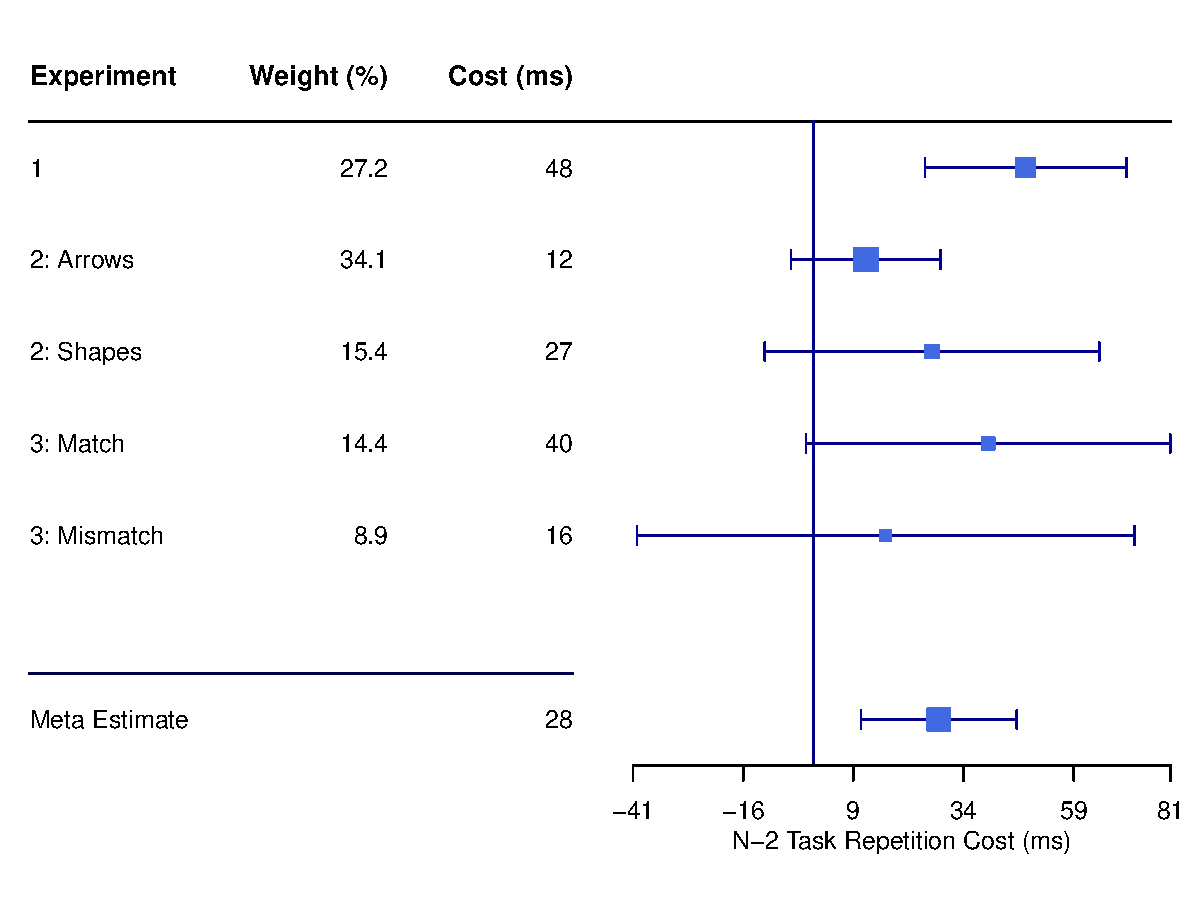
\includegraphics[width = \textwidth]{Images/meta_analysis.pdf}
\caption{Forest plot of the meta-analysis of n--2 task repetition cost for response repetitions across all experiments. The boxes represent the mean n--2 task repetition cost for each condition, together with their 95\% confidence intervals. The size of each box is proportional to that condition's weight in the meta-analysis. The meta-analysis estimate of the n--2 repetition cost is shown at the bottom. Forest plot created using the \texttt{forestplot} R package \citep{Gordon2016}.}
\label{fig:meta_analysis}
\end{center}
\end{figure*}

The result of this meta analysis is shown in Figure \ref{fig:meta_analysis}; the meta-analysis estimate of the n--2 task repetition cost for response repetitions is 28ms, 95\% confidence interval = [11--46ms]. Thus, the evidence across all of our data suggests that there is a small n--2 task repetition cost when controlling for episodic retrieval. As this cost cannot be contaminated by episodic interference from n--2, it is plausible that this estimate is attributable to inhibition. Our data therefore have not provided evidence that episodic retrieval can explain the n--2 task repetition cost entirely, but rather that it reduces the cost considerably. 

\subsection{Conclusion}
In conclusion, our results demonstrate clear effects of episodic interference in generating n--2 task repetition costs, which must be controlled if researchers wish to use this cost as a measure of cognitive inhibition. 









 





\newpage
%%%--------------------------------------------------------------------------------------------
\appendix
\section{Details of Stopping Rules}
In this section we outline the stopping rules for all three experiments. 

\subsection{Experiment 1}
Our sample size for Experiment 1 was determined via optional stopping, utilising Sequential Bayes Factors \citep{Schoenbrodtinpress} to determine our stopping rule for participant recruitment. We were interested in establishing the presence or absence of an interaction between Task Sequence (ABA vs. CBA) and Response Repetition (repetition vs. switch). For the purposes of our stopping rule, this can be expressed as a default within-subjects Bayesian \emph{t}-test \citep{Rouder2009} comparing n--2 task repetition costs for response repetitions and response switches.  We conducted a Bayesian \emph{t}-test on the data collected until the criterion for our a priori stopping rule was met. Specifically, our stopping rule required at least 20 participants; we continued data collection until $BF_{10}$ > 6 (constituting support for the alternative hypothesis) or $BF_{10}$ < 1/6 (constituting support for the null). \cite{Schoenbrodtinpress} demonstrated that a stopping rule of $BF_{10}$ > 6 (or $BF_{10}$ < 1/6) provided the best balance between type 1 and type 2 error, and was their recommended value for studies utilising Sequential Bayes Factors. 

\subsection{Experiment 2}
\subsubsection{Overview of Bayesian analysis of factorial designs}
Experiment 2 again utilised Sequential Bayesian Analysis, but unlike Experiment 1's Bayesian t-test, Experiment 2 utilised Bayesian analysis of factorial designs, outlined by \cite{Rouderinpress} and \cite{Morey2015}. Bayesian analysis of factorial designs generally works by constructing permutations of model comparisons, where the models differ in their inclusion of main effect terms and their interaction. For example, one model might model the data as a main effect of Factor A and a main effect of Factor B, whereas a second model might model the data as a main effect of Factors A and B, as well as their interaction. A Bayes factor is obtained for each model, and the relative evidence for a model comparison is the ratio of their Bayes factors. The result is itself a Bayes factor, which can be used to provide evidence for the degree of support for one model compared to another.

Bayesian analysis for multi-factorial designs can produce hundreds if not thousands of model comparisons \citep[see][]{Rouderinpress}; for example, a 4-factor design has 32,767 model comparisons. Experiment 2 has three factors, so to reduce the number of model comparisons being made we used the n--2 repetition cost as our dependent variable (which removes one factor---Task Sequence---from the design). Thus, the Bayesian factorial analysis had two manipulated factors: Cue-Type and Response Repetition. Participants were entered as a random effect. The Bayes factor for all models was a comparison against a denominator of the n--2 repetition cost predicted by the random effect of participants.

\subsubsection{Stopping rule}
The main model of interest is the model with all main effects and the interaction (i.e., n--2 repetition cost predicted from Cue-Type, Response Repetition, and Cue-Type * Response Repetition interaction). Our stopping rule involved taking the ratio of the Bayes factor for this ``full'' model with the Bayes factor of the next-best model, if the full model had the highest Bayes factor (i.e., if the full model was the best fit, we wished to quantify how much better it is than its nearest competitor). If the full model did not have the highest Bayes factor, we took the ratio of the Bayes factor for the full model with the model with the highest Bayes factor (i.e., if the full model was not the best fit, we wished to quantify how much worse it is than the best model).

Like Experiment 1, our stopping rule required at least 20 participants, and we used a $BF_{10}$ > 6 or $BF_{10}$ < 1/6 as our criterion for stopping data collection. 



\subsection{Experiment 3}
The stopping rule for Experiment 3 was identical to Experiment 2; the factors for this Experiment were Stimulus Condition and Response Repetition; n--2 repetition cost again served as the dependent variable.


%%%--------------------------------------------------------------------------------------------
\appendix
\section{Supplemental Bayesian Analysis for Experiment 1}

\subsection{Visualisation of Sequential Bayesian Analysis} 
The progression of the Bayes Factor for the interaction of Task Sequence and Response Repetition---updated as participants were recruited (see Appendix A for the general procedure)---is shown in Figure \ref{fig:bayesFactor}. We stopped data collection after 76 participants, as at this point the criteria for our stopping rule had been reached. We could have stopped after 75 participants, but the last two participants were tested in successive sessions, so the Bayes factor was not checked until after the final participant. 

\begin{figure*}
\begin{center}
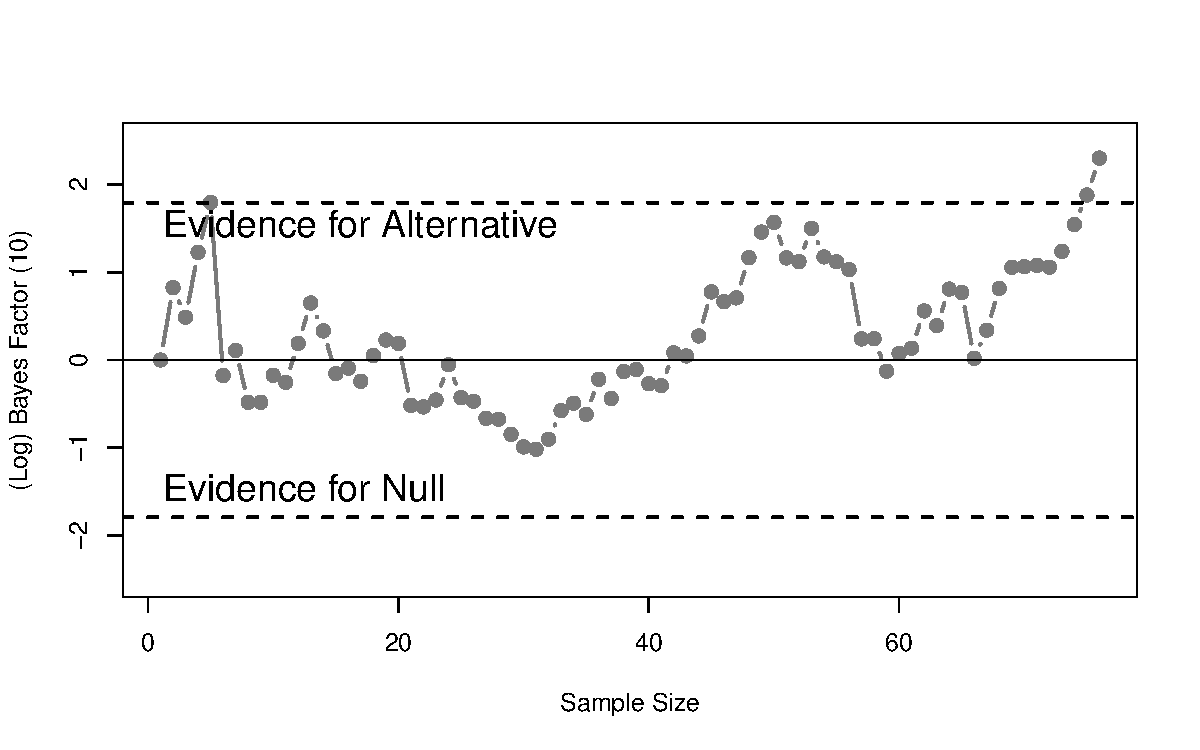
\includegraphics[width = \textwidth]{Images/bayesFactor.pdf}
\caption{Progression of the Sequential Bayes Factor [expressed as log($BF_{10}$)] as sample size increased in Experiment 1. The criteria for a priori stopping rules are shown as dotted horizontal lines.}
\label{fig:bayesFactor}
\end{center}
\end{figure*}

\subsection{Robustness Check on Bayesian Priors}
We used a default prior distribution on the effect size for the alternative hypothesis in the Bayes factor analysis of the critical interaction, which was assumed to be distributed as a Cauchy distribution with scale parameter $r$ = 0.707. To examine how robust our findings were to the choice of prior, we conducted a robustness check by re-calculating the Bayes factor across a wide range of priors by varying scale parameter $r$: As $r$ increases, the prior distribution becomes wider, reflecting a prior for larger effects; $r$ values closer to zero make the distribution narrower, reflecting a prior for smaller effects. The robustness check is plotted in Figure \ref{fig:robustPrior}. This figure shows our conclusions (and our stopping rule) are robust to the prior used: Evidence favours the alternative hypothesis across all plausible prior widths.

\begin{figure*}
\begin{center}
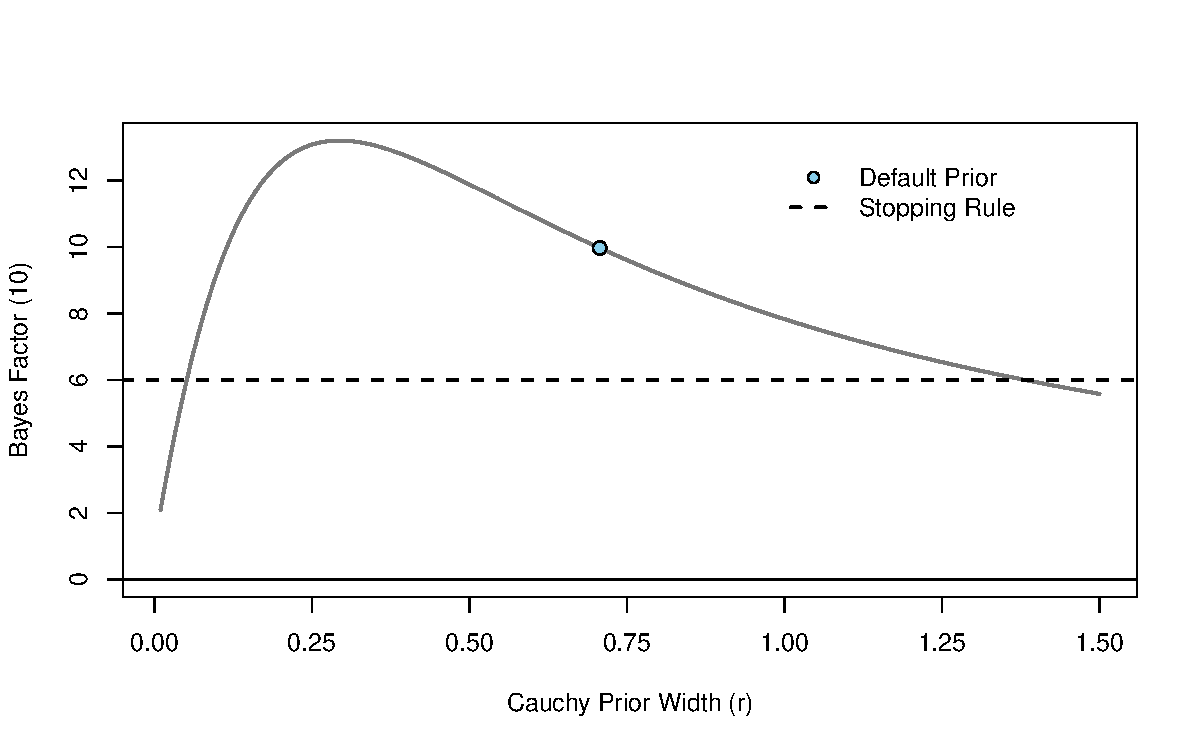
\includegraphics[width = \textwidth]{Images/robustPrior.pdf}
\caption{Robustness check of Bayes factor across a wide range of priors for Experiment 1.}
\label{fig:robustPrior}
\end{center}
\end{figure*}


\subsection{Robustness of Recruitment Order on the Sequential Bayes Factor}
The progression of the Bayes Factor as sample size increased (Figure \ref{fig:bayesFactor}) appeared to provide slight evidence in favour of the null between sample sizes of 30 and 40, although the criterion for stopping was not reached. One might wonder, therefore, whether had a few more participants been recruited to the experiment showing a null interaction would we have stopped data collection and found evidence in favour of the null? Put another way, did recruitment order bias our results?

We wanted to assess how robust our stopping rule was to this apparent early evidence in favour of the null. Specifically, we were interested in whether our stopping rule in favour of the null would have been met had the participants been recruited in a different order. To assess this, we generated 50 random recruitment orders from our data set, and plotted the Sequential Bayes Factors for each recruitment order. If our findings are robust against recruitment order, the stopping rule in favour of the null should be rarely (if ever) met.  The results of this simulation are shown in Figure \ref{fig:recruitmentOrder}; each line represents the Sequential Bayes Factor for a random recruitment order. As can be seen, the stopping criterion in favour of the null is never met, suggesting our results are indeed robust to recruitment order. 

\begin{figure*}
\begin{center}
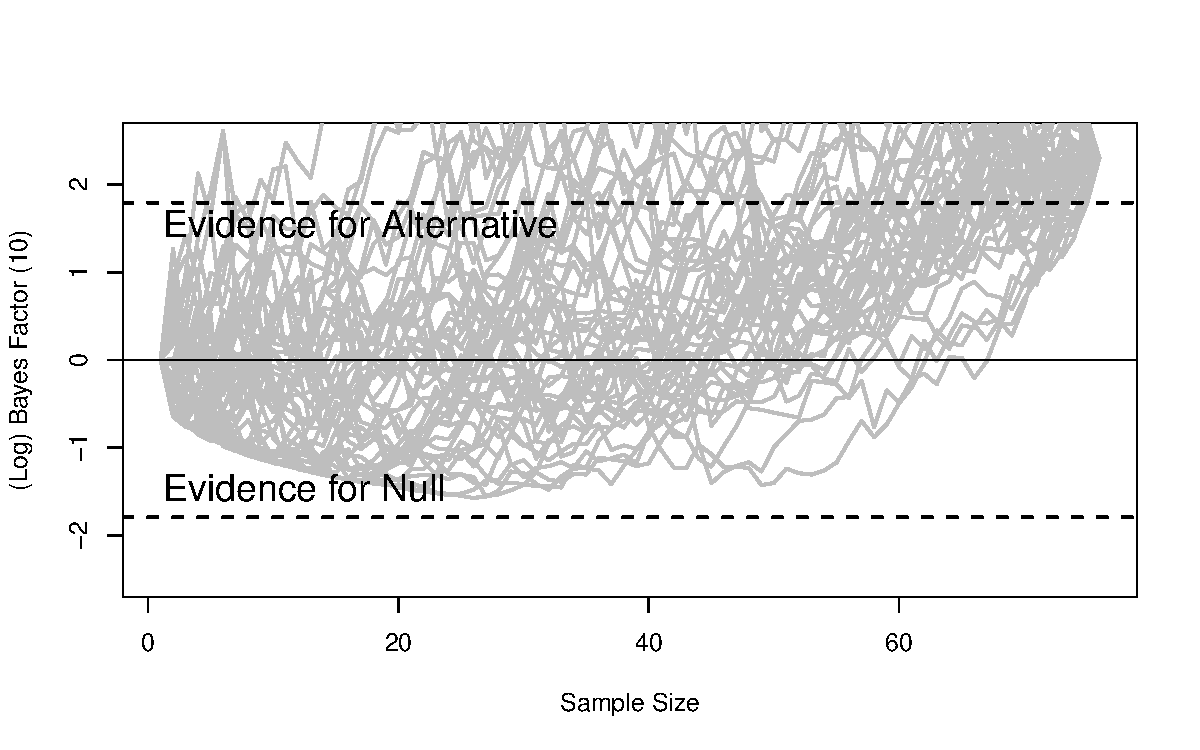
\includegraphics[width =  \textwidth]{Images/recruitmentOrder.pdf}
\caption{Simulated progression of the Sequential Bayes Factors for a random set of 50 different recruitment orders for the current data set in Experiment 1.}
\label{fig:recruitmentOrder}
\end{center}
\end{figure*}

\subsection{Bayesian Parameter Estimation}
Due to the theoretical importance of our main result, we wished to supplement our Bayes factor analysis with Bayesian parameter estimation of the mean and effect size of the difference in n--2 task repetition cost between n--2 response repetitions and response switches. As such, we used the (default) methods outlined by \cite{Kruschke2013}. The input to the analysis was the n--2 task repetition cost for response repetitions minus the n--2 task repetition cost for response switches. The posterior distributions for mean difference and effect size of difference (Cohen's $d$) are shown in Figure \ref{fig:bayesParameter}.

\begin{figure*}
\begin{center}
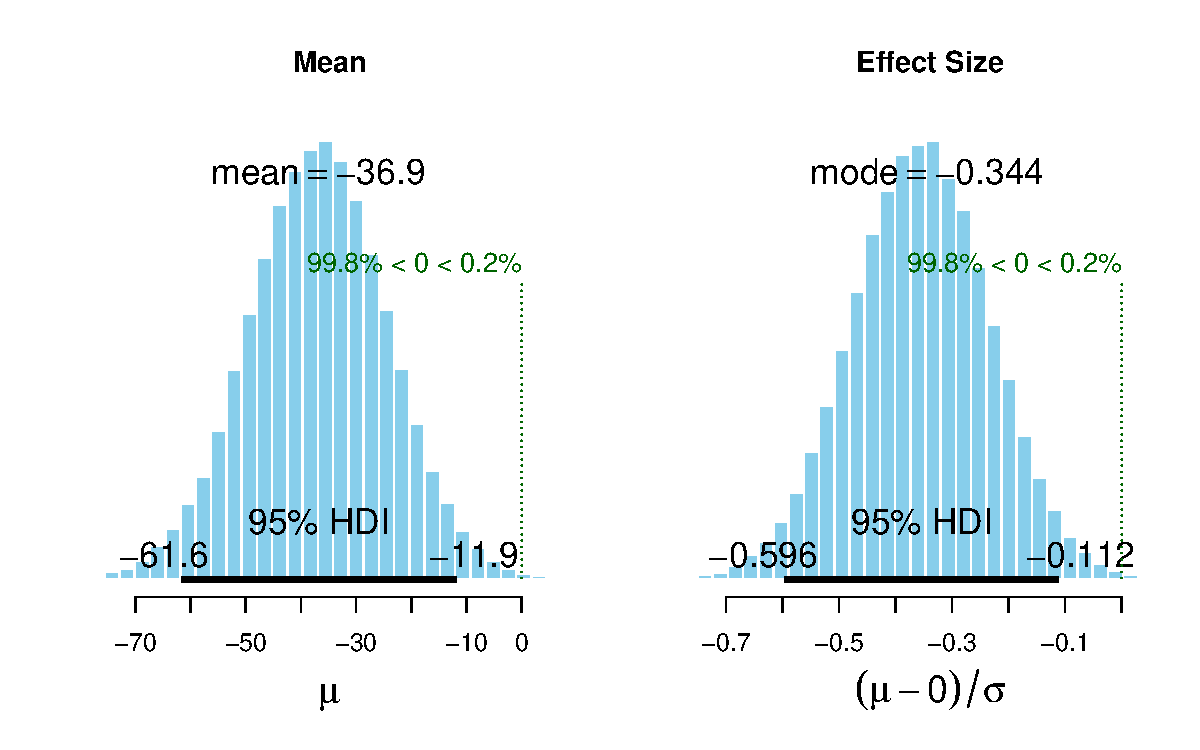
\includegraphics[width = \textwidth]{Images/bayesParameter.pdf}
\caption{Bayesian posterior distributions for the parameters of mean difference and effect size of difference for n--2 task repetition cost [response repetition] minus n--2 task repetition cost [response switch] from Experiment 1. HDI = Highest Density Interval.}
\label{fig:bayesParameter}
\end{center}
\end{figure*}

These posterior distributions present histograms of the Bayesian posterior estimate of the true mean and effect size underlying the data we obtained. The black horizontal bar represents the 95\% Highest Density Interval (HDI); in contrast to frequentist confidence intervals, we can interpret this interval as the range of parameter values we are 95\% certain the true underlying parameter lies within. The mean difference in n--2 task repetition costs for n--2 response repetitions and response switches is estimated to be -37ms; the HDI does not cross zero, so we can be confident that there is a difference between response repetitions and switches. Note, though, that the effect size of this difference is in the small range. 


%%%--------------------------------------------------------------------------------------------
\bibliography{References.bib}

\end{document}
